%
% This is the LaTeX template file for lecture notes for EE 382C/EE 361C.
%
% To familiarize yourself with this template, the body contains
% some examples of its use.  Look them over.  Then you can
% run LaTeX on this file.  After you have LaTeXed this file then
% you can look over the result either by printing it out with
% dvips or using xdvi.
%
% This template is based on the template for Prof. Sinclair's CS 270.

\documentclass[twoside]{article}
\usepackage{graphicx}
\usepackage{wrapfig}
\usepackage{amsmath}
\usepackage{amssymb}
\usepackage{listings}
\setlength{\oddsidemargin}{0.25 in}
\setlength{\evensidemargin}{-0.25 in}
\setlength{\topmargin}{-0.6 in}
\setlength{\textwidth}{6.5 in}
\setlength{\textheight}{8.5 in}
\setlength{\headsep}{0.75 in}
\setlength{\parindent}{0 in}
\setlength{\parskip}{0.1 in}

%
% The following commands set up the lecnum (lecture number)
% counter and make various numbering schemes work relative
% to the lecture number.
%
\newcounter{lecnum}
\renewcommand{\thepage}{\thelecnum-\arabic{page}}
\renewcommand{\thesection}{\thelecnum.\arabic{section}}
\renewcommand{\theequation}{\thelecnum.\arabic{equation}}
\renewcommand{\thefigure}{\thelecnum.\arabic{figure}}
\renewcommand{\thetable}{\thelecnum.\arabic{table}}

%
% The following macro is used to generate the header.
%
\lstset{language=Python, numbers=left, tabsize=2, xleftmargin=5.0ex}

\newcommand{\lecture}[4]{
   \pagestyle{myheadings}
   \thispagestyle{plain}
   \newpage
   \setcounter{lecnum}{#1}
   \setcounter{page}{1}
   \noindent
   \begin{center}
   \framebox{
      \vbox{\vspace{2mm}
    \hbox to 6.28in { {\bf EE 382V: Parallel Algorithms
                        \hfill Summer 2017} }
       \vspace{4mm}
       \hbox to 6.28in { {\Large \hfill Lecture #1: #2  \hfill} }
       \vspace{2mm}
       \hbox to 6.28in { {\it Lecturer: #3 \hfill Scribe: #4} }
      \vspace{2mm}}
   }
   \end{center}
   \markboth{Lecture #1: #2}{Lecture #1: #2}
   %{\bf Disclaimer}: {\it These notes have not been subjected to the
   %usual scrutiny reserved for formal publications.  They may be distributed
   %outside this class only with the permission of the Instructor.}
   \vspace*{4mm}
}

%
% Convention for citations is authors' initials followed by the year.
% For example, to cite a paper by Leighton and Maggs you would type
% \cite{LM89}, and to cite a paper by Strassen you would type \cite{S69}.
% (To avoid bibliography problems, for now we redefine the \cite command.)
% Also commands that create a suitable format for the reference list.
\renewcommand{\cite}[1]{[#1]}
\def\beginrefs{\begin{list}%
        {[\arabic{equation}]}{\usecounter{equation}
         \setlength{\leftmargin}{2.0truecm}\setlength{\labelsep}{0.4truecm}%
         \setlength{\labelwidth}{1.6truecm}}}
\def\endrefs{\end{list}}
\def\bibentry#1{\item[\hbox{[#1]}]}

%Use this command for a figure; it puts a figure in wherever you want it.
%usage: \fig{NUMBER}{SPACE-IN-INCHES}{CAPTION}
\newcommand{\fig}[3]{
			\vspace{#2}
			\begin{center}
			Figure \thelecnum.#1:~#3
			\end{center}
	}
% Use these for theorems, lemmas, proofs, etc.
\newtheorem{theorem}{Theorem}[lecnum]
\newtheorem{lemma}[theorem]{Lemma}
\newtheorem{proposition}[theorem]{Proposition}
\newtheorem{claim}[theorem]{Claim}
\newtheorem{corollary}[theorem]{Corollary}
\newtheorem{definition}[theorem]{Definition}
\newenvironment{proof}{{\bf Proof:}}{\hfill\rule{2mm}{2mm}}

% **** IF YOU WANT TO DEFINE ADDITIONAL MACROS FOR YOURSELF, PUT THEM HERE:

\begin{document}
%FILL IN THE RIGHT INFO.
%\lecture{**LECTURE-NUMBER**}{**DATE**}{**LECTURER**}{**SCRIBE**}
\lecture{2}{June 9}{Vijay Garg}{Eric Addison}
%\footnotetext{These notes are partially based on those of Nigel Mansell.}

% **** YOUR NOTES GO HERE:

% Some general latex examples and examples making use of the
% macros follow.  
%**** IN GENERAL, BE BRIEF. LONG SCRIBE NOTES, NO MATTER HOW WELL WRITTEN,
%**** ARE NEVER READ BY ANYBODY.
\section{Introduction}
During this lecture, we were exposed to the first parallel algorithm of the class (a simple array sum). We continued with this example to introduce and explore some of the fundamental concepts in parallel algorithm construction and analysis, including:
\begin{itemize}
	\item the \texttt{•}{reduce} operation
	\item parallel algorithm metrics (time, work, cost)
	\item Brent's Scheduling Principle
	\item Work-Optimal Algorithms
\end{itemize}

This set of lecture notes will briefly re-examine the topics covered in this lecture, in the order in which they appeared during class.

\section{The \texttt{reduce} Operation}
A \texttt{reduce} operation, for the purposes of this lecture, refers to the process of ``reducing" a collection of values to a single result, presumably through the application of an \textit{associative} binary operation. For example, consider an array of values \texttt{A} and a binary operation $*$ (standard multiplication, perhaps). Performing the \texttt{reduce} operation on \texttt{A}, in this case, is equivalent to:
\[
r = \texttt{reduce}(\texttt{A},*) = \texttt{A}[1]*\texttt{A}[2]*\texttt{A}[3]* ... *\texttt{A}[N]
\]
Common \texttt{reduce} operations include minimum, maximum, sum, and product.

Associativity is desired so that the operation can be distributed among separate threads for parallel execution. Recall that a binary operation $*$ is associative if $a*(b*c) = (a*b)*c$.

\section{Parallel Algorithm Metrics}
Next, we took a few minutes so each of us could write an implementation of a simple array sum. Naturally, most of us wrote down about three to five lines of code to implement the trivial $O(n)$ sequential solution:
\begin{lstlisting}
s:=0;
for i:=0 to n-1 do
	s:= s + A[i];
\end{lstlisting}

As most of us know, this algorithm has time complexity $O(n)$ for an array of size $n$. We denote the time complexity by $T(n)$, i.e.:
\begin{center}
$T(n) \equiv$ the time complexity of an algorithm with input size $n$
\end{center}

For parallel algorithms, we are also interested in a new quantity called \textit{work}, denoted $W(n)$:
\begin{center}
$W(n) \equiv$ the work required for an algorithm with input size $n$
\end{center}

The work required by an algorithm was explained by the \textit{Work-Depth Model of Computation}. 
 
 
\subsection{Work-Depth Model of Computation} 
\begin{wrapfigure}[4]{r}{0.3\textwidth}
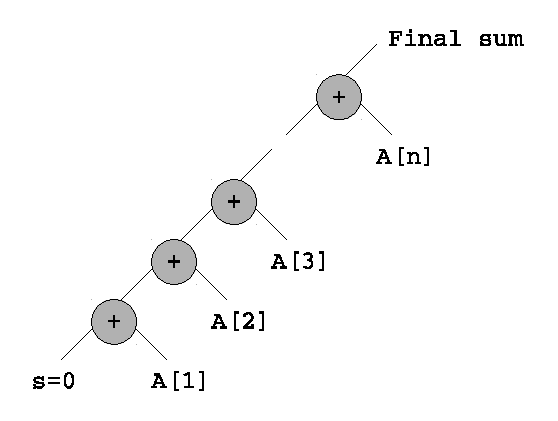
\includegraphics[scale=0.7]{img/wd_model_1.eps}
\end{wrapfigure}

The work-depth model consists of a directed acyclic graph (DAG) that represents the computation. For the sequential \texttt{reduce}-sum algorithm, the DAG looks like the figure on the right. In the model, each level of the graph represents one time step, so the running time is equal to the depth of the graph. We then have the following relationships:
\begin{itemize}
	\item depth = time required on a parallel machine
	\item work = number of nodes in the graph
\end{itemize}
So here we have $W(n) = O(n)$.

\subsection{Parallel Sum} \label{sec:parSum}
How can we improve on the sequential algorithm? We must adjust our thinking to move away from the old fashioned coding style of the 1960s and 70s, and start thinking in a 21st century way. Assume we have $p$ processors available. The big question becomes:
\begin{center}
\boxed{\text{Can we arrange the work in a binary tree?}}
\end{center}
Consider an array of length eight. The work-depth model can be arranged as a binary tree as follows:
\begin{figure}[h]
\center
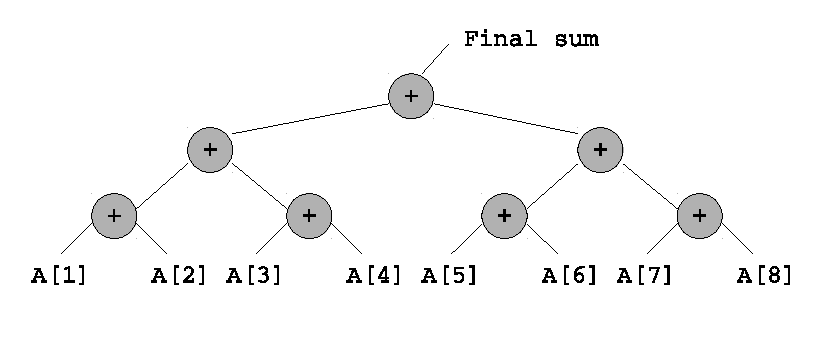
\includegraphics[scale=0.75]{img/wd_model_2} 
\end{figure}

We assign one processor to each of the graph nodes along the bottom of the tree (assume $p\geq 8$ for the moment). Since each level of the tree takes one time step to complete, we have parallel metrics $T(n) = O(\log n)$ (depth of tree) and $W(n) = O(n)$ (number of nodes). And of course, we know that reducing the time complexity from $O(n)$ to $(\log n)$ is a *big* deal!

\section{Brent's Scheduling Principle}
What if we have fewer than $n$ processors available, i.e. $p<n$? Then we cannot assign each node along the bottom row of the work-depth model tree to a single processor. The required time $T(n,p)$ for an algorithm with a problem of size $n$ on $p$ processors is given by \textbf{BRENT'S SCHEDULING PRINCIPLE}, i.e.:
\[
T(n,p) = \frac{W(n)}{p} + T(n),
\]
where $T(n)$ is the depth of the work-depth model. We can prove that this is true.

\textbf{Proof:} Time to simulate level $i$ of the work-depth model with $p$ processors is
\[
\left\lceil\frac{W^{i}(n)}{p}\right\rceil \leq \frac{W^{i}(n)}{p} + 1,
\]
where $W^{i}(n)$ is the work required at level $i$ of the model. The total running time is the sum of all the level times:
\begin{align*}
T(n,p) &\leq \sum_{i=1}^{T(n)}\left( \frac{W^{i}(n)}{p} + 1 \right) \\
	&= \frac{1}{p}\sum_{i=1}^{T(n)}W^{i}(n) + \sum_{i=1}^{T(n)}1\\
	&= \frac{W(n)}{p} + T(n)
\end{align*}

The first line of the previous block of equations is an inequality, however when we work in asymptotic quantities, this can be disregarded and the strict equality of Brent's Scheduling Principle is valid. More formally, we might want to write $T(n,p) = O\left(\frac{W(n)}{p} + T(n)\right)$.
\begin{flushright}
$\Box$
\end{flushright}

Consider the previous sum example with $p = O(n/\log n)$. We then have parallel run time:
\begin{align*}
T(n,p) 	&= \dfrac{O(n)}{O(n/\log n)} + O(\log n)\\
		&= O\left(\dfrac{n}{n/\log n} + \log n\right)\\
		&= O(\log n)
\end{align*}
This implies that in order to compute a \texttt{reduce} operation in $O(\log n)$ time, we only need $O(n/\log n)$ processors! (not $O(n)$!)

\subsection{Cost}
We also defined a fourth parallel metric, the \textit{cost}, with $C(n,p) = T(n,p)\cdot p$, though we did not discuss it much in this lecture.


\section{Work-Optimal Algorithms}
Let $T_{\text{seq}}(n)$ be the best case sequential time complexity for some problem. A parallel algorithm $\mathcal{A}$ is said to be \textbf{WORK OPTIMAL} if its required work $W(n) = O(T_{\text{seq}}(n))$.

\subsection{Cascading}
Next we will use the notion of \textit{cascading} two algorithms together to achieve work optimality. Consider breaking the array \texttt{A} up into $n/\log n$ segments of size $\log n$:
\begin{figure}[h]
\center
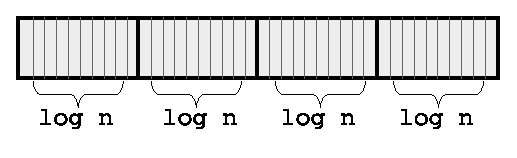
\includegraphics[scale=1]{img/split_array}
\end{figure}

The cascade technique works by applying an algorithm $\mathcal{A}$ with the desired work complexity to each of the segments (where $\mathcal{A}$ could be sequential or parallel), and then applying a parallel algorithm $\mathcal{B}$ on the results. For example, let's say that $\mathcal{A}$ is a sequential algorithm with $T_{\mathcal{A}}(n) = O(n)$ and $W_{\mathcal{A}}(n) = O(n)$, and $\mathcal{B}$ is a non-optimal parallel algorithm with $T_{\mathcal{B}}(n) = O(\log n)$ and $W_{\mathcal{B}}(n) = O(n\log n)$. The cascade technique proceeds as:
\begin{align*}
\textbf{step 1: }& \text{run $\mathcal{A}$ on each segment}\\
& \qquad \text{Total time complexity } T(n) = O(\log n) \\
& \qquad \text{Total work complexity } W(n) = O(n)\\
&\\
\textbf{step 2: }& \text{run $\mathcal{B}$ on the segment results}\\
& \qquad \text{Total time complexity } T(n) = O(\log(n/\log n)) < O(\log n) \\
& \qquad \text{Total work complexity } W(n) = O(n/\log n \cdot \log(n/\log n)) < O(n)\\
\\
\textbf{Total Complexity: }& \text{sum of step 1 and step 2 complexities}\\
& \qquad \text{Total time complexity } T(n) = O(\log n) + O(\log n)  = O(\log n)\\
& \qquad \text{Total work complexity } W(n) = O(n) + O(n) = O(n)
\end{align*}

Use of the cascade technique in this case has produced a work complexity of $O(n)$, which makes it a work optimal algorithm. Cool!

\pagebreak
\section{More Parallel \texttt{reduce} Analysis}

See the official course lecture notes for a convenient table comparing complexities of different algorithms.

\subsection{Parallel \texttt{reduce}-sum: Binary Tree}
The initial parallel algorithm we examined for the \texttt{reduce}-sum problem was to rearrange the work-depth model into a binary tree (instead of a ``stupid" tree): see section \ref{sec:parSum}. A pseudo-code implementation of this algorithm is:
\begin{lstlisting}
i:= get_my_id();
B[i]:= A[i]
for h:= 1 to log n do
	if (i <= n/(2^h)) then
		B[i]:= B[2i-1] + B[2i];
print B[1];
\end{lstlisting}

Assume 1-based array indexing. By relying on the lock-step feature of our PRAM model, this implementation builds the binary tree upward by overwriting array entries on the left side of the array at each time step, finally producing the sum at position \texttt{B[1]}. The complexity of this algorithm is:
\[
T(n) = O(\log n),\qquad W(n) = O(n)
\]

Since the best case sequential time for \texttt{reduce}-sum is $T_{\text{seq}}(n) = O(n)$, this algorithm is \textbf{work optimal}.

\subsection{Parallel \texttt{reduce}-sum: Network Models}
\begin{wrapfigure}[12]{r}{0.3\textwidth}
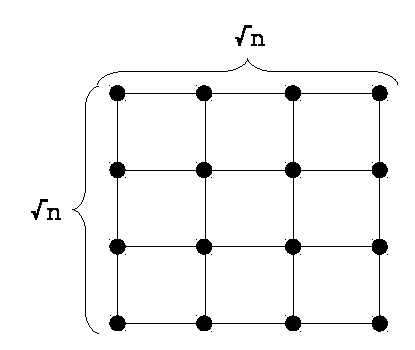
\includegraphics[scale=0.75]{img/mesh.eps}
\end{wrapfigure}

What if we change our parallel computation model? We can visualize a 2D mesh network of $n$ nodes by constructing a $\sqrt{n} \times \sqrt{n}$ grid as shown on the right. If we perform the sum by summing across all rows (in parallel), and then down along one column, the resulting complexities are
\[
T(n) = O(\sqrt{n}),\qquad W(n) = O(n)
\]
If the network is arranged as a hypercube of dimension $d$, and the sum is performed by summing along one dimension at a time, then the complexities become:
\[
T(n) = O(\log{n}),\qquad W(n) = O(n)
\]


\subsection{Parallel \texttt{reduce}-max: All Pairs}
Can we achieve a better time complexity than $O(\log n)$ for a \texttt{reduce} operation? Note that our previous attempts only made use of an EREW PRAM model ... no concurrent reads or writes were needed. Consider evaluating the \texttt{reduce}-max operation on a common-CRCW machine. In this case, it is possible to achieve a time complexity of $O(1)$! This is done with a parallel technique known as \textbf{all pairs}. 

Instead of utilizing only $n$ processors for this problem of size $n$, let's use $n^2$. Essentially we will use one processor to perform each of the $n^2$ possible comparisons. An array \texttt{isBiggest} will be initialized to all \texttt{true} values, and all but the actual max value will attempt to change the corresponding array value to \texttt{false}. Pseudo-code for this algorithm follows:
\begin{lstlisting}
for all i parallel do
	isBiggest[i]:= true

for all i,j: i!=j parallel do
	if(A[j]>A[i])
		isBiggest[i]:= false

for all i parallel do
	if isBiggest[i]
		max:= A[i]

\end{lstlisting}

Since each of the \texttt{for} loops are performed completely in parallel, each loop has time complexity $T_{\text{loop}}(n) = O(1)$, and so the total time is also $O(1)$. Unfortunately, the loop over $i,j$ results in $O(n^2)$ work, so this algorithm, while very time efficient, is not work-optimal.

\subsection{Parallel \texttt{reduce}-max: Doubly Logarithmic}
Clearly we can't do better than $T(n) = O(1)$ for time complexity, but we can still do better by finding a work-optimal algorithm. Consider again the \texttt{reduce}-max problem of size $n$, and imagine dividing the $n$ elements into $\sqrt{n}$ segments of size $\sqrt{n}$. Take each of those new segments and split each of them in the same way, i.e. each segment of size $n^{1/2}$ will be split into $n^{1/4}$ new segments of size $n^{1/4}$, and so on. This splitting can be visualized in a tree:
\begin{figure}[h]
\center
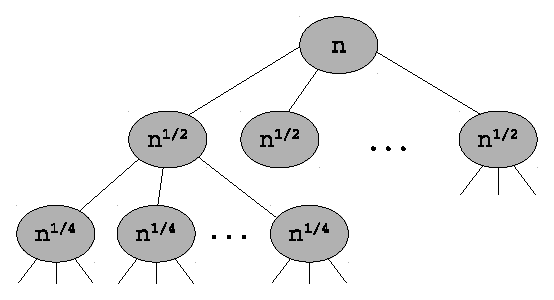
\includegraphics[scale=1]{img/doublelogtree.eps}
\end{figure}

At the $i^{\text{th}}$ level of the tree (for $i>0$), there are $\prod_{j=1}^{i}n^{2^{-j}}$ segments containing $n^{2^{-i}}$ elements each. We can confirm that there are still $n$ elements at every level:
\[
n^{2^{-i}}\prod_{j=1}^{i}n^{2^{-j}} = n^{2^{-i} + \sum_{j=1}^{i}2^{-j}} = n^{2^{-i} - 1 + \frac{1-2^{-i-1}}{1-1/2}} = n^{2^{-i}-1+2-2^{-i}} = n
\]
How many levels of the tree are there? Assume that the original size $n=2^{2^{h}}$. After $i$ splits, each segment contains $n_i = (2^{2^{h}})^{2^{-i}} = 2^{2^{h}2^{-i}} = 2^{2^{h-i}}$. After $h$ levels, there will be $2^{2^{0}}=2$ elements per segment, the tree cannot be split any further, so we can say the tree has height $h$. With a work-depth model that has depth $h$, if we can evaluate the max at each level of the tree in $O(1)$ time (we can do this with the all-pairs algorithm), then the time complexity is given by the relation of $h$ to $n$, namely:
\[
T(n) = O(h) = O(\log \log n)
\]

This is a \textit{doubly logarithmic} time complexity, and is really really good! For some sense of the smallness of the double log, assume a tree height of $h=10$ (a pretty small run time). This corresponds to an input of size $2^{2^{10}} \sim O(10^{300})$, a positively \textit{huge} number! 

For work complexity, notice that each level of the tree requires $O(n)$ work. Consider tree level $i$, where we will use the all-pairs algorithm locally at each tree node to compute the max of its children. At this level, each node must aggregate the results from its $n_{\text{ch}}^i = n^{2^{-i-1}}$ children. The all-pairs algorithm then results in time $T_{\text{node}}^i(n) = O(1)$ and requires $(n_{ch}^{i})^2$ work. This must be done for all $N^{i}_{\text{nodes}} = \prod_{j=1}^{i}n^{2^{-j}}$ nodes at a given level, so the total work required for level $i$ is:
\[
W^{i}(n) = O((n_{ch}^{i})^{2}N^{i}_{\text{nodes}}) = O\left(n^{2^{-i}} \prod_{j=1}^{i}n^{2^{-j}}\right) = O(n)
\]
And, if the work at every level is $W^{i}(n) = O(n)$, then the cumulative work at all depths is
\[
W(n) = O(n\log n \log n),
\]
which means this algorithm is \textit{not} work-optimal.

\subsection{Parallel \texttt{reduce}-max: Cascaded Doubly Logarithmic (optimal)}
By applying the cascade technique to the doubly logarithmic tree, we can describe a very efficient work-optimal algorithm for \texttt{reduce}-max. Referring back to the section on cascading, let's assign algorithm $\mathcal{A}$ as the standard $O(n)$ sequential algorithm, and algorithm $\mathcal{B}$ as the doubly logarithmic algorithm. This time, split the initial array into $N_{\text{seg}} = O(n/(\log \log n))$ segments of size $n_{\text{seg}} = O(\log \log n)$. Now the cascade technique proceeds as:
\begin{align*}
\textbf{step 1: }& \text{run $\mathcal{A}$ on each segment (in parallel)}\\
& \qquad \text{Total time complexity } T(n) = O(\log \log n) \\
& \qquad \text{Total work complexity } W(n) = O(n/(\log \log n))*O(\log \log n) = O(n)\\
&\\
\textbf{step 2: }& \text{run $\mathcal{B}$ on the segment results}\\
& \qquad \text{Total time complexity } T(n) = O(\log \log(n/(\log \log n))) < O(\log \log n) \\
& \qquad \text{Total work complexity } W(n) = O(n/(\log \log n) * \log \log(n/(\log \log n))) < O(n)\\
&\\
\textbf{Total Complexity: }& \text{sum of step 1 and step 2 complexities}\\
& \qquad \text{Total time complexity } T(n) = O(\log \log n) + O(\log \log n)  = O(\log \log n)\\
& \qquad \text{Total work complexity } W(n) = O(n) + O(n) = O(n)
\end{align*}
This is a \textbf{work-optimal}, efficient algorithm for the \texttt{reduce}-max problem. Since we use the all-pairs algorithm as part of the doubly logarithmic algorithm, it is written for a common-CRCW PRAM model.


\end{document}





